\newpage % Rozdziały zaczynamy od nowej strony.
\section{Generowanie podpisów do obrazów -- aktualne rozwiązania}
W celu wygenerowania podpisu do obrazu przy użyciu algorytmów uczenia maszynowego wykorzystuje się sieci neuronowe. Sam proces generowania podpisów można rozbić na dwa etapy: przetwarzanie obrazu oraz generowanie tekstu. Z tego względu najpopularniejsze podejścia wykorzystują połączenia sieci wykorzystywanych do przetwarzania obrazów wraz z sieciami wykorzystywanymi do przetwarzania języka naturalnego. Takie podejście wyodrębnia dwa główne moduły w całej architekturze sieci:
\begin{itemize}
  \item moduł kodujący obraz -- jego danymi wejściowymi jest obraz w postaci macierzy pikseli, natomiast wyjściem jest wektor sprowadzony do postaci zgodnej z formatem wejściowym modułu dekodującego,
  \item moduł dekodujący zakodowany obraz wcześniej obraz -- wejściem tego modułu jest wyjście modułu kodującego, natomiast wyjściem jest ostatecznie wygenerowane zdanie.
\end{itemize}
\begin{figure}[H]
  \centering
  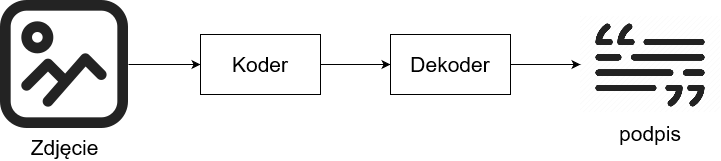
\includegraphics[width=.9\linewidth]{diagram}
  \caption{Typowa architektura generatora podpisów. Opracowanie własne}
  \label{fig:schemat-captioning}
\end{figure}
\subsection{Moduły kodujące}
Ze względu na niezwykle dużą skuteczność, jak również popularność, najczęściej wykorzystywaną siecią neuronową jako moduł kodujący jest splotowa sieć neuronowa. Główną jej modyfikacją, w celu dostosowania do problemu, jakim jest generowanie podpisów, jest dopasowanie ostatnich warstw w taki sposób, aby~ostateczny wektor wyjściowy był kompatybilny z typowym formatem danych wejściowych sieci wykorzystywanych w dziedzinie przetwarzania języka naturalnego.
\subsubsection{Bardzo głębokie sieci splotowe}
Jednym z częściej wykorzystywanych rodzajów sieci splotowej są głębokie sieci neuronowe. Charakteryzują się one dużą liczbą warstw splotowych oraz małymi wielkościami filtrów. Aktualnie istnieje wiele architektur wykorzystujących takie podejście. Jedną z pierwszych była sieć VGGNet \cite{vggnet}. Dzięki zastosowaniu dużej liczby warstw splotowych możliwe było klasyfikowanie obrazów o dużej rozdzielczości z bardzo wysoką skutecznością. Dużym minusem tego rodzaju sieci są wymagane zasoby. Ze względu na dużą ilość warstw konieczna jest alokacja duże ilości pamięci w jednostce GPU, a samo przetworzenie danych przez sieć wymaga wielu obliczeń.
\subsubsection{Transformer wizyjny}
Transformer wizyjny \cite{vit} to model przetwarzania obrazów, który różni się od tradycyjnych architektur zawierających sieci splotowe. Opiera się on na transformerze znanym głównie z zastosowań w przetwarzaniu języka naturalnego. Przy jego pomocy obraz jest przetwarzany poprzez podzielenie na nienachodzące się bloki, a każdy blok reprezentowany jest jako token, podobnie jak słowa w zdaniu. Te tokeny są traktowane jako sekwencja wejściowa dla modelu transformera. Poglądowy diagram przedstawiający architekturę transformera wizyjnego został przedstawiony na rysunku \ref{fig:vit-architecture}.
\begin{figure}[H]
  \centering
  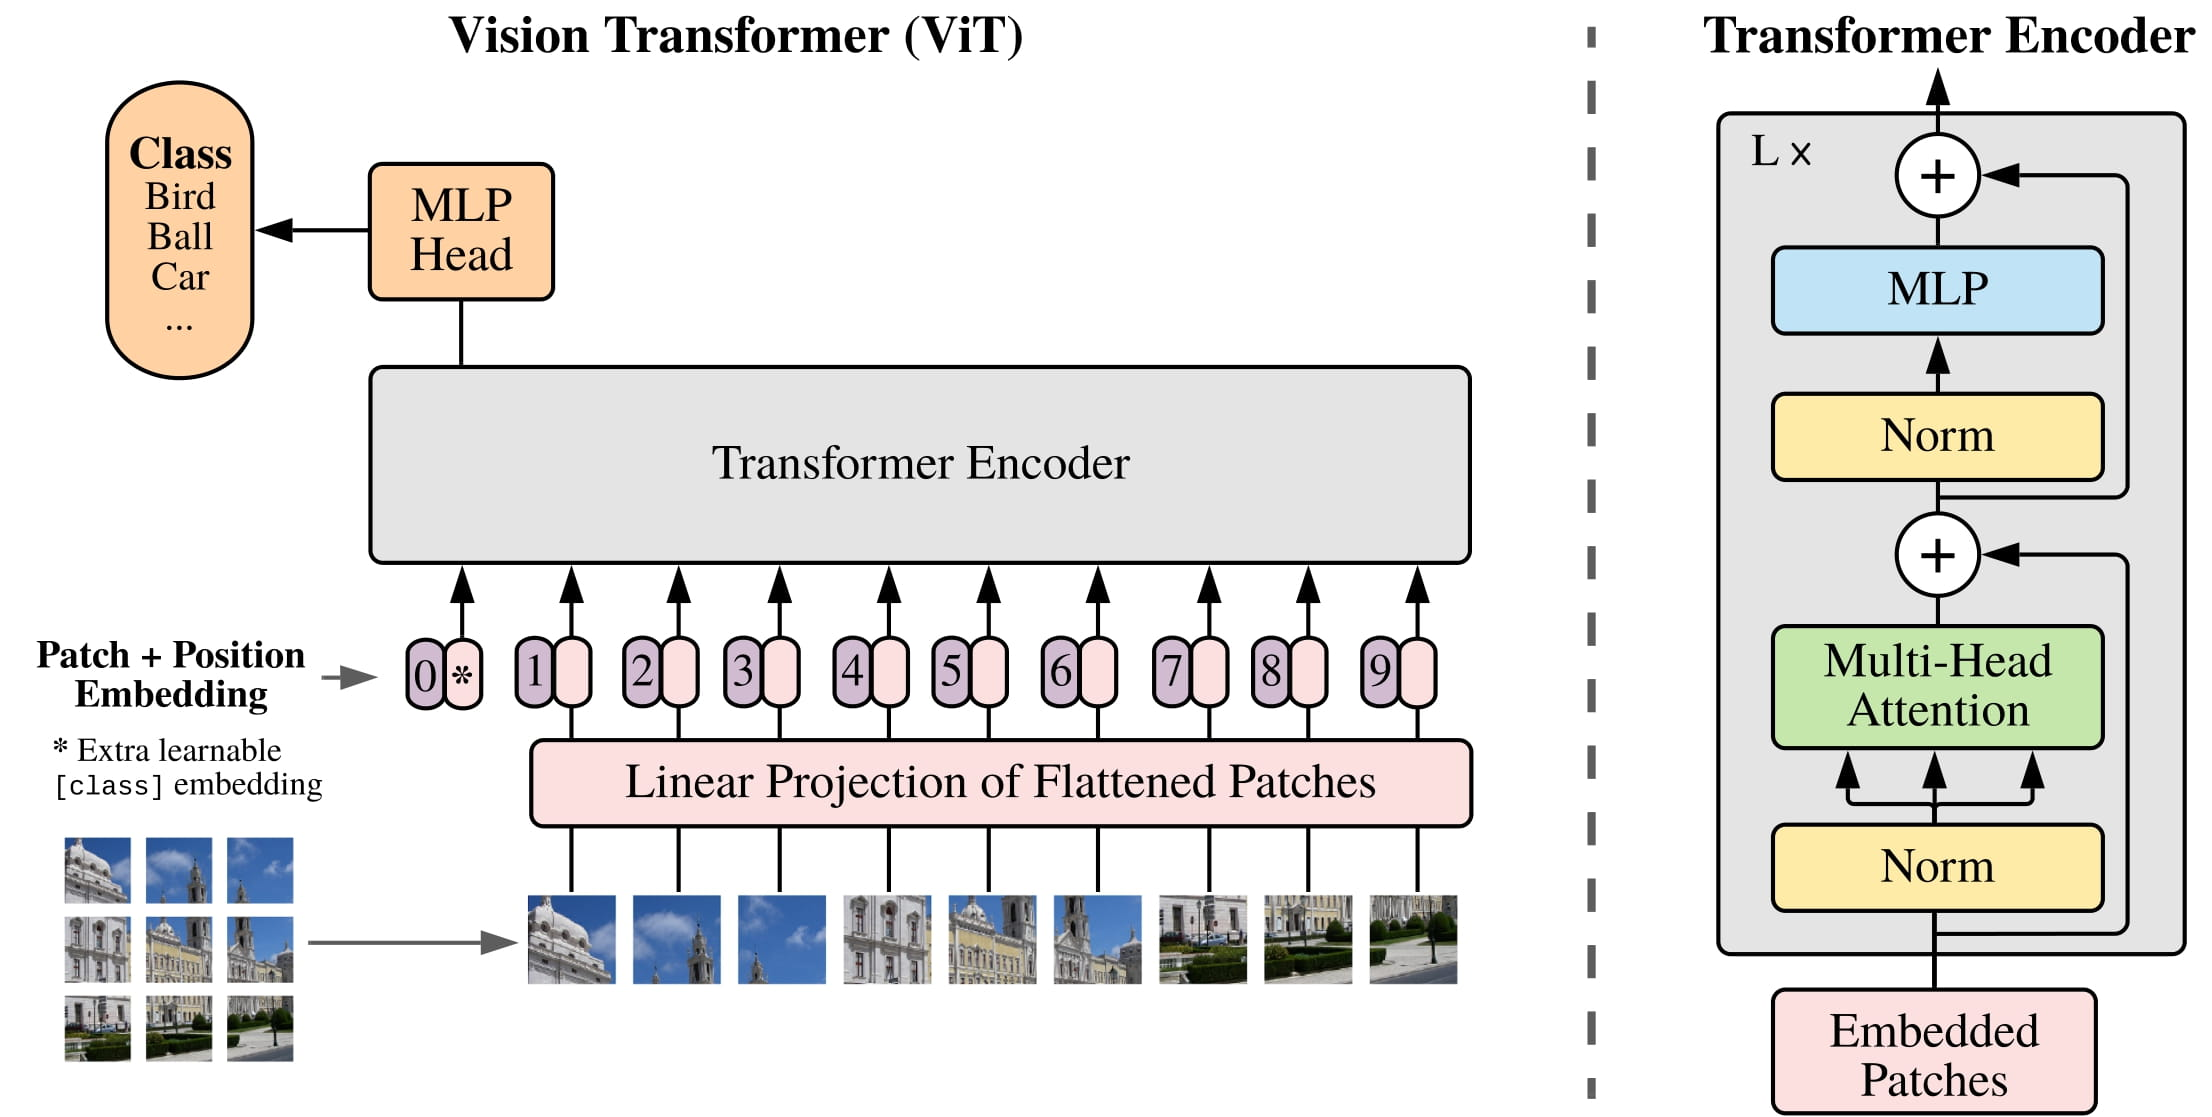
\includegraphics[width=.95\linewidth]{vit_architecture}
  \caption{Diagram architektury transformera wizyjnego. Źródło: \cite{vit}}
  \label{fig:vit-architecture}
\end{figure}
\noindent Dane wyjściowe z kodera transformera przetwarzane są w bardzo podobny sposób jak w przypadku danych wyjściowych głębokich warstw sieci splotowych -- przy pomocy w pełni połączonych warstw, wektor wyjściowy jest sprowadzany do postaci wektora zawierającego odpowiednie klasy, co zostało przedstawione na diagramie przy pomocy bloku ,,MLP Head'' oraz ,,Class''.
\subsection{Moduły dekodujące}
Dzięki sprowadzeniu obrazu do formatu zwykłego wektora poprzez moduł kodujący możliwe jest wykorzystanie większości rozwiązań dedykowanych do zwykłych zadań przetwarzania języka naturalnego. Jako analogiczną dziedzinę można tutaj wyróżnić zagadnienie związane z generowaniem odpowiedzi na pytania -- główną różnicą w przypadku generowania podpisów jest sprowadzenie obrazu do wartości możliwe do przetworzenia przez moduł kodujący. W przypadku zagadnień związanych z generowaniem odpowiedzi, przetwarzany jest tekst, natomiast w przypadku generowania podpisów są to obrazu. Dalsza część architektury, czyli moduł kodujący, jest analogiczna w obu przypadkach. Częstym wyborem jest podstawowa rekurencyjna sieć neuronowa. W przypadku takiej sieci wektor będący wyjściem modułu kodującego służy jako pierwszy element wejściowy moduły dekodującego. Naturalnie możliwe jest wykorzystywanie bardziej zaawansowanych odmian sieci rekurencyjnej jak LSTM oraz GRU. Również wykorzystywane są moduły atencji, w których przypadku szczególnie użyteczne są głębokie sieci neuronowe. Wyniki z poprzednich warstw splotowych służą jako kontekst, z którego może korzystać moduł atencji.
\subsubsection{Transformer}
% MAYBE rozwinąć
Tak jak w przypadku pozostałych problemów związanych z przetwarzaniem języka naturalnego, również w kontekście generowania podpisów do obrazów, popularnością cieszy się sieć Transformer \cite{transformer}. Jest to niezwykle skomplikowana architektura, jednakże możliwość użycia jej wcześniej wytrenowanych wag, w celu dostrojenia modelu pod wybrane zadanie, bardzo usprawnia cały proces wytwarzania rozwiązania.
\subsection{Przykład architektur}
Architektura NIC (ang. Neural Image Caption) \cite{nic} wykorzystuje połączenie splotowej sieci neuronowej oraz sieć LSTM, w celu generowania podpisów. Osiąga ona wartość BLEU-4 na poziomie 27,7 dla zbioru MS COCO \cite{mscoco}.

Bardziej rozbudowana architektura GIT (ang. Generative Image-to-text Transformer) \cite{wang2022git} na zbiorze danych MS COCO osiągnęła wartość metryki BLEU-4 równą 43,2 -- wynik o 50\% lepszy. Wykorzystuje ona model Transformera wizyjnego jako moduł kodujący wraz z klasycznym Transformerem wykorzystanym jako moduł dekodujący. Rozwiązanie to pochodzi z 2022 roku i aktualnie osiąga jedne z najlepszych wyników w dziedzinie generowania podpisów do obrazków.

Architektura OFA (ang. Once for all) \cite{wang2022ofa} została stworzona z myślą o wielozadaniowości, dzięki czemu jest w stanie rozwiązać wiele zadań związanych z przetwarzaniem obrazów cyfrowych, w tym generowania podpisów. Model ten nie jest ograniczony jedynie do przetwarzania obrazów, ponieważ opiera się on na metodzie seq2seq, polegającej na przetwarzanie pewnej sekwencji do innej sekwencji. Jego danymi wejściowymi są dane językowy, którym może towarzyszyć obraz, z tego względu oprócz macierzy pikseli danego obrazka konieczne również jest podanie tekstu w postaci formuły informującej architekturę o konieczności wygenerowania podpisu jak na przykład „co opisuje obraz?”. Wszelkie typy zadań rozwiązywane przez architekturę OFA zostały zobrazowane na rysunku \ref{fig:ofa-tasks} stworzonym przez autorów sieci.
\begin{figure}[H]
  \centering
  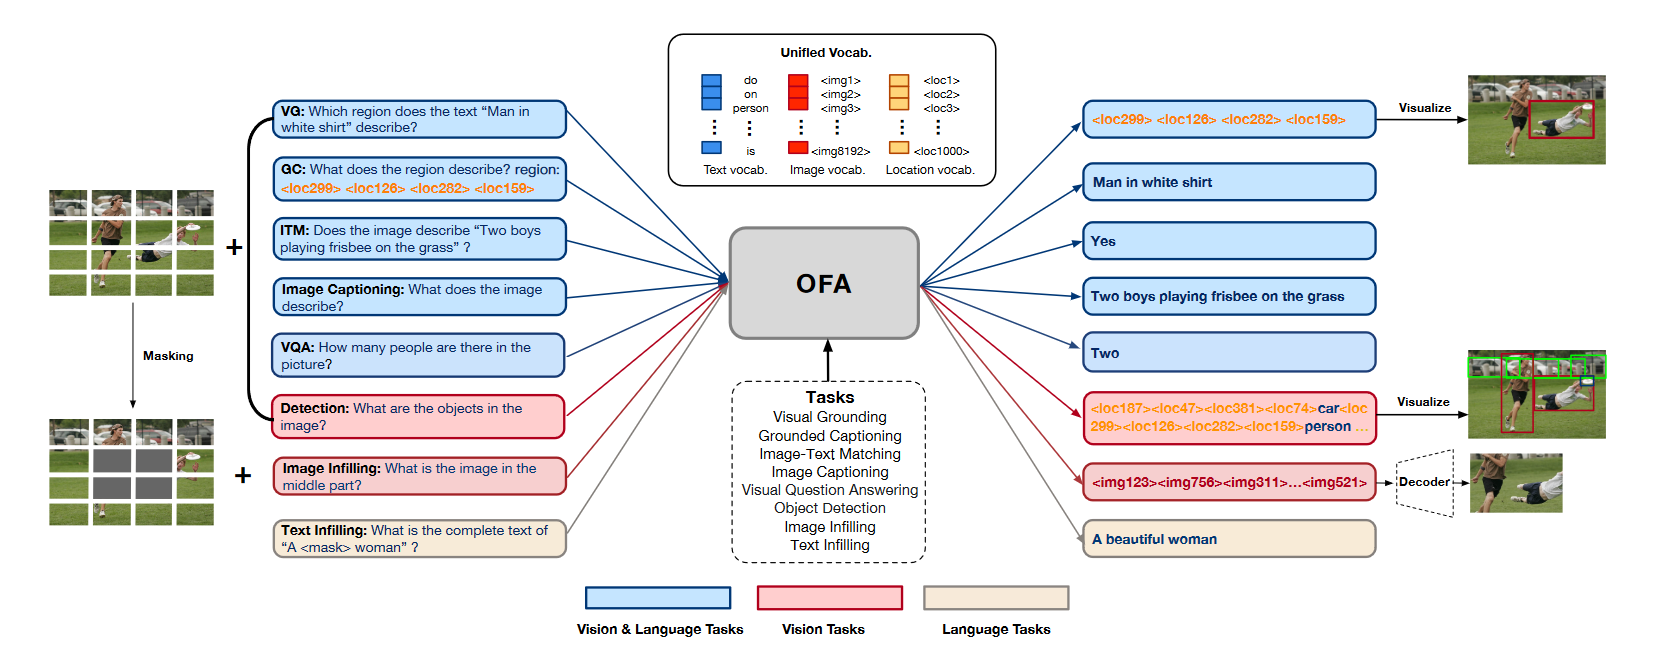
\includegraphics[width=\linewidth]{ofa_tasks}
  \caption{Diagram przedstawiający możliwe typy zadań rozwiązywane przez architekturę OFA. Źródło: \cite{wang2022ofa}}
  \label{fig:ofa-tasks}
\end{figure}
% MAYBE opisać technikalia architektury OFA 
\subsection{Wydajność aktualnych rozwiązań}
Publikowanych jest coraz więcej artykułów dotyczących uczenia maszynowego, jednakże ciężko jest znaleźć publikacje podejmujące problem, jakim są wysokie wymagania sprzętowe potrzebne do stworzenia takiego rozwiązania, jak również jego wykorzystywania. Najczęściej w przypadku opisywania autorskiej architektury sieci neuronowej, autorzy podają ramy czasowe poświęcone na trenowanie architektury wraz z nazwą wykorzystywanej jednostki GPU. O wiele rzadziej pojawia się informacji o samym czasie potrzebnym do przetworzenia pojedynczej wartości wejściowej w kontekście późniejszego wykorzystywania proponowanego rozwiązania.
Przykładem publikacji, które poruszają problem wysokich wymagań sprzętowych rozwiązań dotyczących neuronowych sieci splotowych oraz rekurencyjnych są:
\begin{itemize}
  \item Analiza wydajności splotowych sieci neuronowych bazujących na GPU \cite{cnn-compare},
  \item Optymalizacja wydajności rekurencyjnych sieci neuronowych wykorzystujących GPU \cite{rnn-compare}.
\end{itemize}
Niestety ze względu na o wiele mniejszą popularność dziedziny generowania podpisów do obrazków, ciężko znaleźć badania dotyczące konkretnie tego problemu. W łatwy sposób można oszacować, w jaki sposób zmieniać będzie się sama wydajność wykorzystywanych architektur poprzez połączenie czasów jednego modułu wraz z czasami drugiego modułu otrzymanymi z w istniejących badaniach. Mimo wszystko takich wyników nie można uznać za dokładne ze względu na konieczność wprowadzenia modyfikacji w konkretnych architekturach modułów. Dodatkowym problemem jest brak informacji o skuteczności danej architektur w kontekście zastosowanych zasobów.
